% Options for packages loaded elsewhere
\PassOptionsToPackage{unicode}{hyperref}
\PassOptionsToPackage{hyphens}{url}
\PassOptionsToPackage{dvipsnames,svgnames,x11names}{xcolor}
%
\documentclass[
  letterpaper,
  DIV=11,
  numbers=noendperiod]{scrartcl}

\usepackage{amsmath,amssymb}
\usepackage{iftex}
\ifPDFTeX
  \usepackage[T1]{fontenc}
  \usepackage[utf8]{inputenc}
  \usepackage{textcomp} % provide euro and other symbols
\else % if luatex or xetex
  \usepackage{unicode-math}
  \defaultfontfeatures{Scale=MatchLowercase}
  \defaultfontfeatures[\rmfamily]{Ligatures=TeX,Scale=1}
\fi
\usepackage{lmodern}
\ifPDFTeX\else  
    % xetex/luatex font selection
\fi
% Use upquote if available, for straight quotes in verbatim environments
\IfFileExists{upquote.sty}{\usepackage{upquote}}{}
\IfFileExists{microtype.sty}{% use microtype if available
  \usepackage[]{microtype}
  \UseMicrotypeSet[protrusion]{basicmath} % disable protrusion for tt fonts
}{}
\makeatletter
\@ifundefined{KOMAClassName}{% if non-KOMA class
  \IfFileExists{parskip.sty}{%
    \usepackage{parskip}
  }{% else
    \setlength{\parindent}{0pt}
    \setlength{\parskip}{6pt plus 2pt minus 1pt}}
}{% if KOMA class
  \KOMAoptions{parskip=half}}
\makeatother
\usepackage{xcolor}
\setlength{\emergencystretch}{3em} % prevent overfull lines
\setcounter{secnumdepth}{-\maxdimen} % remove section numbering
% Make \paragraph and \subparagraph free-standing
\makeatletter
\ifx\paragraph\undefined\else
  \let\oldparagraph\paragraph
  \renewcommand{\paragraph}{
    \@ifstar
      \xxxParagraphStar
      \xxxParagraphNoStar
  }
  \newcommand{\xxxParagraphStar}[1]{\oldparagraph*{#1}\mbox{}}
  \newcommand{\xxxParagraphNoStar}[1]{\oldparagraph{#1}\mbox{}}
\fi
\ifx\subparagraph\undefined\else
  \let\oldsubparagraph\subparagraph
  \renewcommand{\subparagraph}{
    \@ifstar
      \xxxSubParagraphStar
      \xxxSubParagraphNoStar
  }
  \newcommand{\xxxSubParagraphStar}[1]{\oldsubparagraph*{#1}\mbox{}}
  \newcommand{\xxxSubParagraphNoStar}[1]{\oldsubparagraph{#1}\mbox{}}
\fi
\makeatother


\providecommand{\tightlist}{%
  \setlength{\itemsep}{0pt}\setlength{\parskip}{0pt}}\usepackage{longtable,booktabs,array}
\usepackage{calc} % for calculating minipage widths
% Correct order of tables after \paragraph or \subparagraph
\usepackage{etoolbox}
\makeatletter
\patchcmd\longtable{\par}{\if@noskipsec\mbox{}\fi\par}{}{}
\makeatother
% Allow footnotes in longtable head/foot
\IfFileExists{footnotehyper.sty}{\usepackage{footnotehyper}}{\usepackage{footnote}}
\makesavenoteenv{longtable}
\usepackage{graphicx}
\makeatletter
\newsavebox\pandoc@box
\newcommand*\pandocbounded[1]{% scales image to fit in text height/width
  \sbox\pandoc@box{#1}%
  \Gscale@div\@tempa{\textheight}{\dimexpr\ht\pandoc@box+\dp\pandoc@box\relax}%
  \Gscale@div\@tempb{\linewidth}{\wd\pandoc@box}%
  \ifdim\@tempb\p@<\@tempa\p@\let\@tempa\@tempb\fi% select the smaller of both
  \ifdim\@tempa\p@<\p@\scalebox{\@tempa}{\usebox\pandoc@box}%
  \else\usebox{\pandoc@box}%
  \fi%
}
% Set default figure placement to htbp
\def\fps@figure{htbp}
\makeatother

\KOMAoption{captions}{tableheading,figureheading}
\makeatletter
\@ifpackageloaded{caption}{}{\usepackage{caption}}
\AtBeginDocument{%
\ifdefined\contentsname
  \renewcommand*\contentsname{Table of contents}
\else
  \newcommand\contentsname{Table of contents}
\fi
\ifdefined\listfigurename
  \renewcommand*\listfigurename{List of Figures}
\else
  \newcommand\listfigurename{List of Figures}
\fi
\ifdefined\listtablename
  \renewcommand*\listtablename{List of Tables}
\else
  \newcommand\listtablename{List of Tables}
\fi
\ifdefined\figurename
  \renewcommand*\figurename{Figure}
\else
  \newcommand\figurename{Figure}
\fi
\ifdefined\tablename
  \renewcommand*\tablename{Table}
\else
  \newcommand\tablename{Table}
\fi
}
\@ifpackageloaded{float}{}{\usepackage{float}}
\floatstyle{ruled}
\@ifundefined{c@chapter}{\newfloat{codelisting}{h}{lop}}{\newfloat{codelisting}{h}{lop}[chapter]}
\floatname{codelisting}{Listing}
\newcommand*\listoflistings{\listof{codelisting}{List of Listings}}
\makeatother
\makeatletter
\makeatother
\makeatletter
\@ifpackageloaded{caption}{}{\usepackage{caption}}
\@ifpackageloaded{subcaption}{}{\usepackage{subcaption}}
\makeatother

\usepackage{bookmark}

\IfFileExists{xurl.sty}{\usepackage{xurl}}{} % add URL line breaks if available
\urlstyle{same} % disable monospaced font for URLs
\hypersetup{
  pdftitle={Global Renewable Energy Leaders in 2023},
  pdfauthor={Arisara Therdthianwong; Quanyu Qian; Dhruv Kaushal Gal},
  colorlinks=true,
  linkcolor={blue},
  filecolor={Maroon},
  citecolor={Blue},
  urlcolor={Blue},
  pdfcreator={LaTeX via pandoc}}


\title{Global Renewable Energy Leaders in 2023}
\author{Arisara Therdthianwong \and Quanyu Qian \and Dhruv Kaushal Gal}
\date{}

\begin{document}
\maketitle

\renewcommand*\contentsname{Table of Contents}
{
\hypersetup{linkcolor=}
\setcounter{tocdepth}{3}
\tableofcontents
}

\subsection{Executive summary}\label{executive-summary}

This report investigates the top 10 countries with the highest renewable
energy share in 2023 and global trends in energy transitions. It further
analyzes the sources of renewable energy in the leading country. The
analysis is conducted using reliable data from Our World in Data. Among
these countries, Norway stands out as a global leader with 72.09\% of
its primary energy coming from renewable sources. The findings offer
valuable insight to effectively implement national approaches that could
transform sustainable energy transitions worldwide.

\newpage

\subsection{Introduction}\label{introduction}

The global energy landscape has transformed rapidly in the last few
decades. Many countries are undergoing a major shift toward adopting
renewable sources such as hydropower, wind, and solar in response to the
challenges of climate change and resource sustainability. Renewable
energy now plays an important role as an alternative source that helps
to reduce reliance on fossil fuels and mitigate greenhouse gas
emissions.

Throughout the report, global renewable energy trends are identified,
with a focus on the top 10 countries with highest proportion of
renewable energy in total energy consumption in 2023. Norway leads the
way, with roughly 72\% of primary energy sourced from renewable. Sweden
and Brazil are also undergoing significant transitions, with 53.9\% and
50.3\% renewable shares, respectively.

A deeper analysis on Norway has been conducted to better understand how
a developed country manages its energy infrastructure achieving a high
level of renewable integration. Understanding these factors behind
Norway's performance can be beneficial for planning and improving
renewable energy policies and strategies that could be adapted to
different regional and national contexts. This analysis aims to provide
a useful insight that can guide future energy transitions globally.

\newpage

\section{Methodology}\label{methodology}

Building on the global patterns identified above, we used 2023 data from
Our World in Data to examine national-level energy composition.
Aggregated regions were excluded to identify the top 10 countries by
renewable energy share.

We focused on Norway---the global leader---to explore the drivers behind
its performance. This included analyzing Norway's internal energy mix,
comparing it with other major economies, and evaluating absolute
hydropower output across countries.

This multi-layered analysis provides both a proportional and
quantitative basis for assessing Norway's global leadership in renewable
energy.

\subsection{Top 10 Countries by Renewable Energy Share in
2023}\label{top-10-countries-by-renewable-energy-share-in-2023}

\begin{longtable}[]{@{}llrr@{}}

\caption{\label{tbl-table-top10}Top 10 Countries by Renewable Energy
Share (\%) in 2023}

\tabularnewline

\toprule\noalign{}
Country & Code & Year & Renewables (\%) \\
\midrule\noalign{}
\endhead
\bottomrule\noalign{}
\endlastfoot
Norway & NOR & 2023 & 72.09110 \\
Sweden & SWE & 2023 & 53.89018 \\
Brazil & BRA & 2023 & 50.33141 \\
Denmark & DNK & 2023 & 42.73486 \\
New Zealand & NZL & 2023 & 42.26695 \\
Austria & AUT & 2023 & 40.08019 \\
Switzerland & CHE & 2023 & 38.32534 \\
Portugal & PRT & 2023 & 36.04341 \\
Finland & FIN & 2023 & 35.93626 \\
South and Central America (EI) & NA & 2023 & 35.39018 \\

\end{longtable}

\begin{figure}

\caption{\label{fig-top10-bar}Bar chart of Top 10 Countries by Renewable
Energy Share (\%) (2023)}

\centering{

\pandocbounded{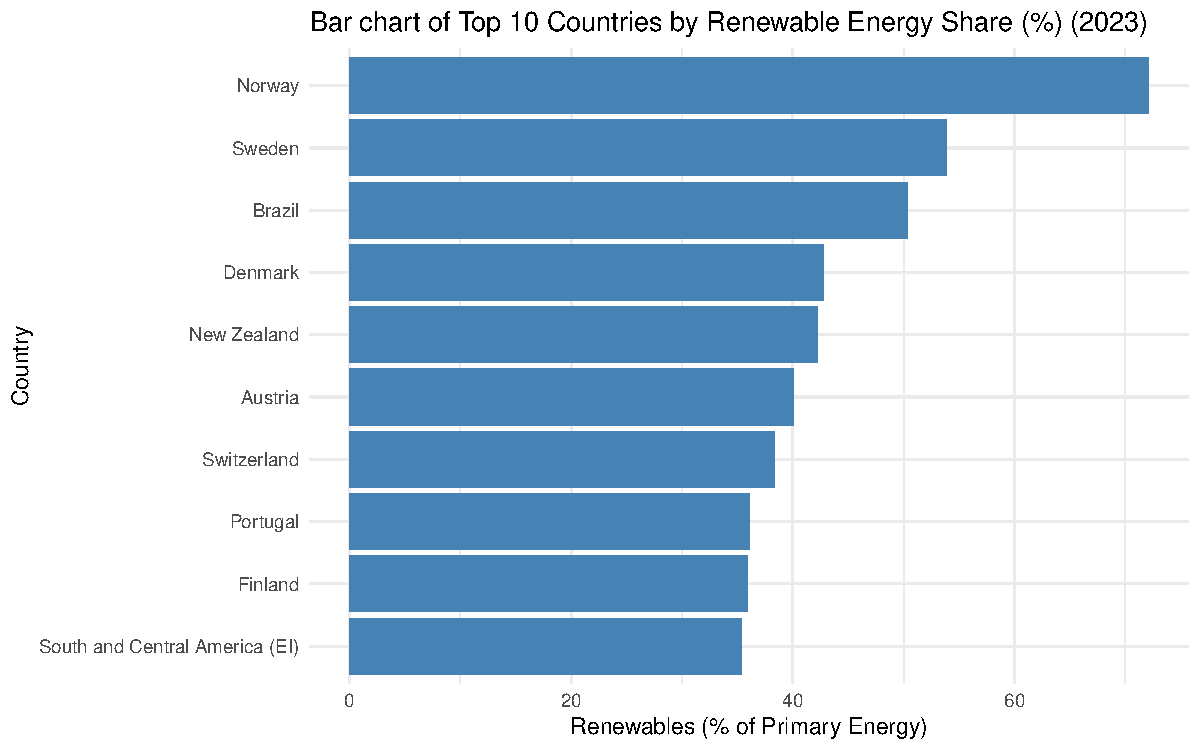
\includegraphics[keepaspectratio]{Assignment3_files/figure-pdf/fig-top10-bar-1.pdf}}

}

\end{figure}%

Table~\ref{tbl-table-top10} and Figure~\ref{fig-top10-bar} show the top
10 countries with the highest renewable energy shares.\\
Norway leads with over 70\%, far ahead of others.

Its standout performance led us to investigate its domestic energy
sources.

\subsection{Norway: Global Leader in
2023}\label{norway-global-leader-in-2023}

To understand Norway's lead, we examined its 2023 electricity mix
(Table~\ref{tbl-table-norway-2023}).

\begin{longtable}[]{@{}lr@{}}

\caption{\label{tbl-table-norway-2023}Norway's Renewable Electricity
Generation by Source in 2023 (TWh)}

\tabularnewline

\toprule\noalign{}
Source & TWh \\
\midrule\noalign{}
\endhead
\bottomrule\noalign{}
\endlastfoot
wind & 14.96 \\
hydro & 135.96 \\
solar & 0.17 \\
Other renewables including bioenergy & 0.26 \\

\end{longtable}

\begin{figure}

\caption{\label{fig-norway-sources}Norway's Renewable Electricity
Breakdown by Source in 2023 (TWh)}

\centering{

\pandocbounded{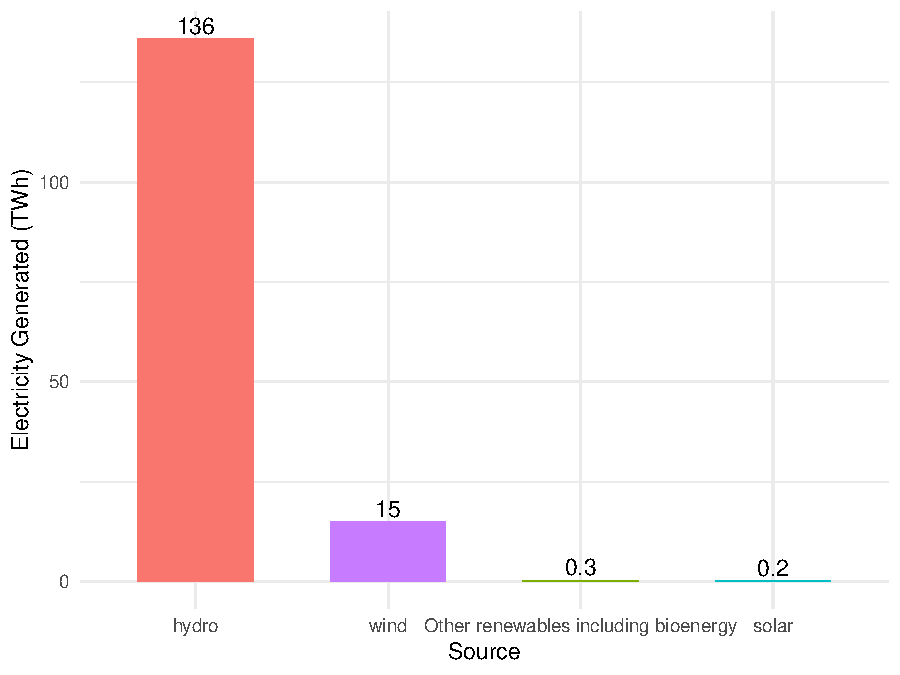
\includegraphics[keepaspectratio]{Assignment3_files/figure-pdf/fig-norway-sources-1.pdf}}

}

\end{figure}%

As shown in Figure~\ref{fig-norway-sources}, hydropower generated 136
TWh---over 90\% of its renewable output---while wind contributed 15 TWh.
Solar and bioenergy were minimal.

This indicates Norway's dominance stems from heavy reliance on
hydropower, rather than a diverse mix of renewable sources.

\subsection{Global Hydropower Generation by Country
(2023)}\label{global-hydropower-generation-by-country-2023}

A high renewable share may not indicate real capacity.

To determine whether its leadership is substantive, we further compared
Norway's absolute hydropower output with that of other major economies.

\begin{figure}

\caption{\label{fig-global-hydro}Global Hydropower Generation (TWh) in
2023 by Country}

\centering{

\pandocbounded{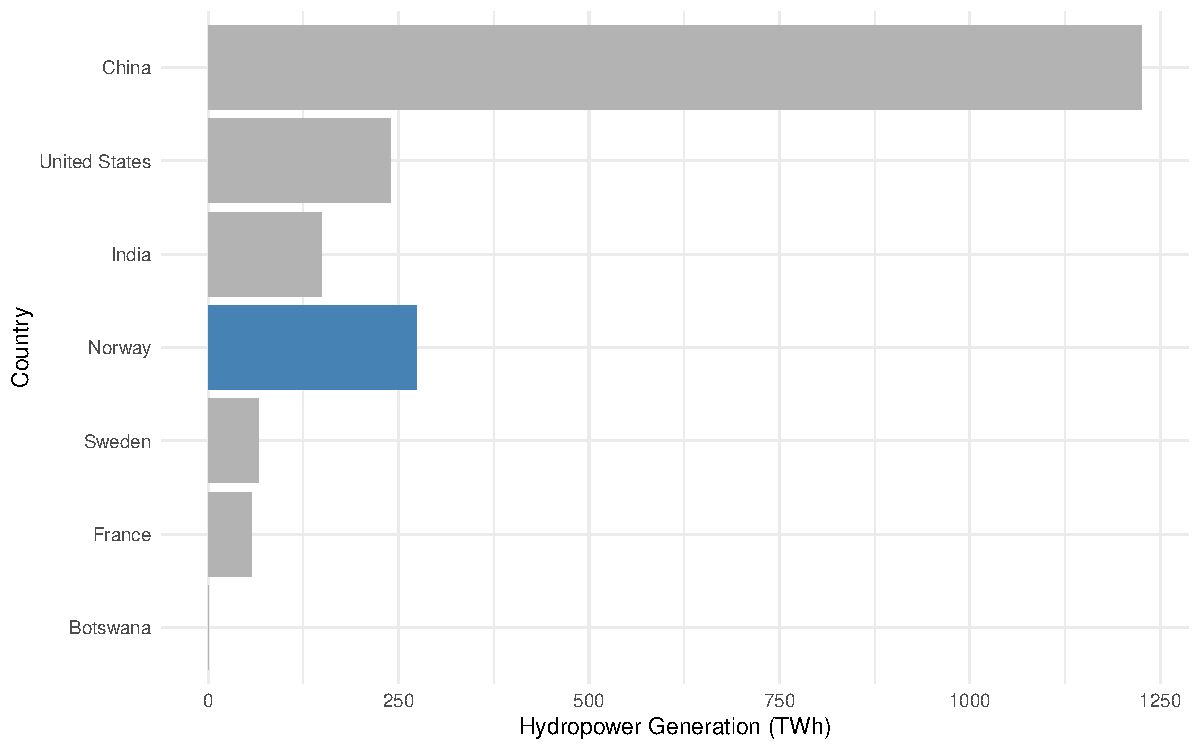
\includegraphics[keepaspectratio]{Assignment3_files/figure-pdf/fig-global-hydro-1.pdf}}

}

\end{figure}%

Figure~\ref{fig-global-hydro} shows that in 2023, Norway generated 270
TWh---exceeding the U.S. (239 TWh) and India (149 TWh), despite its
significantly smaller population and land area.

This demonstrates that Norway's leadership in renewable energy is not
just based on proportional share, but is firmly supported by substantial
infrastructure and high absolute output in clean energy production.

\section{Results}\label{results}

The analysis revealed that in 2023, Norway led globally in renewable
energy adoption, with 72.09\% of its primary energy coming from
renewable sources, as shown in Table~\ref{tbl-table-top10}. Sweden
(53.9\%) and Brazil (50.3\%) followed closely, highlighting strong
national commitments to clean energy transitions.

Figure~\ref{fig-top10-bar} visualizes these rankings, with Norway's
share standing distinctly above the rest of the top 10. This
outperformance reflects long-term national investments and natural
hydroelectric potential.

To understand this further, Table~\ref{tbl-table-norway-2023} and
Figure~\ref{fig-norway-sources} show that Norway's 2023 electricity mix
was over 90\% hydropower, supported by modest wind output and minimal
solar and bioenergy contributions.

Crucially, Figure~\ref{fig-norway-trend} illustrates that Norway's
leadership is not new---it has maintained a renewable share above 60\%
for over two decades. This trend reinforces the country's sustained
commitment to renewable development through stable policy, investment,
and infrastructure planning.

Overall, these results demonstrate that top-performing countries combine
favorable geography with long-term national strategies. Norway
exemplifies how consistent planning and natural resource optimization
can produce a globally leading clean energy profile.

\begin{figure}

\caption{\label{fig-norway-trend}Norway's Renewable Energy Share
(2000--2023)}

\centering{

\pandocbounded{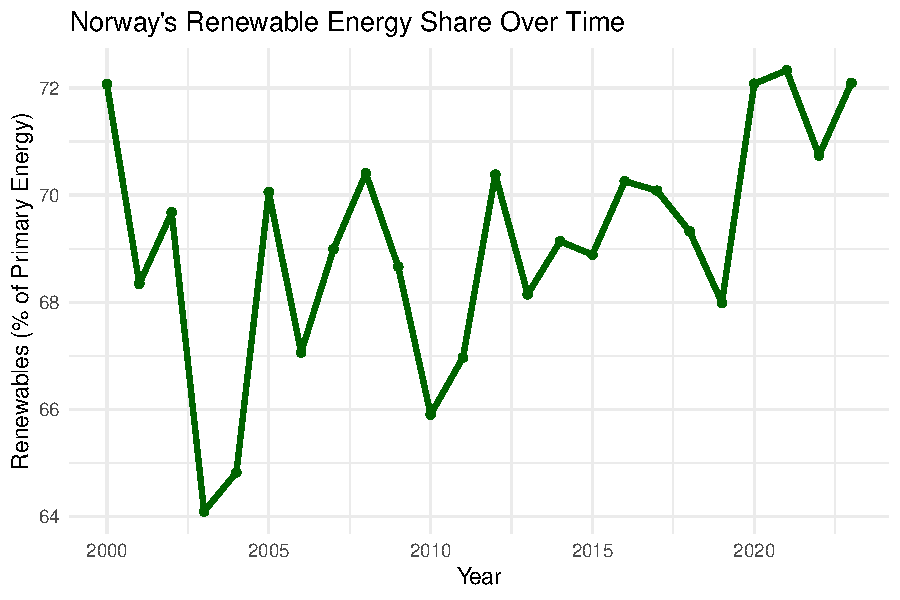
\includegraphics[keepaspectratio]{Assignment3_files/figure-pdf/fig-norway-trend-1.pdf}}

}

\end{figure}%

\section{Discussion and Conclusion}\label{discussion-and-conclusion}

Norway's top ranking in renewable energy share is not incidental---it
reflects decades of strategic investment in hydroelectric
infrastructure, supported by favorable geography and a stable policy
environment. The country's energy profile, dominated by hydropower,
illustrates how natural endowments can be effectively leveraged to
transition away from fossil fuels.

However, this reliance on a single dominant source introduces potential
vulnerabilities. Climate variability, such as droughts or shifting
precipitation patterns, could significantly impact hydroelectric
generation. Furthermore, despite its leadership, Norway's use of wind,
solar, and bioenergy remains minimal, indicating untapped potential for
diversification.

The global comparison in hydropower generation reinforces Norway's
substantial absolute output relative to its size. This combination of
high renewable share and high volume is rare among countries and
highlights the effectiveness of long-term, resource-aligned energy
planning.

In conclusion, Norway's case exemplifies how geographic advantages, when
matched with consistent national policy and infrastructure investment,
can result in world-leading performance in renewable energy integration.

\subsubsection{Recommendations}\label{recommendations}

\begin{itemize}
\tightlist
\item
  \emph{Diversify energy sources}: Invest in wind and solar to reduce
  overreliance on hydropower.
\item
  \emph{Modernize energy infrastructure}: Improve grid flexibility to
  integrate more variable renewables.
\item
  \emph{Export expertise}: Share Norway's policy, regulatory, and
  engineering frameworks with other nations.
\item
  \emph{Support adaptive policy}: Prepare for climate risks by
  developing redundancy and storage solutions.
\end{itemize}

\subsection{References}\label{references}

Our World in Data. (2024). Renewable energy data explorer. Retrieved
from \url{https://ourworldindata.org/renewable-energy}

Our World in Data. (2024). Hydropower generation by country. Retrieved
from \url{https://ourworldindata.org/grapher/hydropower-consumption}

\subsection{Citations}\label{citations}

Library readr - Wickham H, Hester J, Bryan J (2024). \emph{readr: Read
Rectangular Text Data}. R package version 2.1.5,
https://github.com/tidyverse/readr, \url{https://readr.tidyverse.org}.

Library Tidyverse - Wickham H, Averick M, Bryan J, Chang W, McGowan LD,
François R, Grolemund G, Hayes A, Henry L, Hester J, Kuhn M, Pedersen
TL, Miller E, Bache SM, Müller K, Ooms J, Robinson D, Seidel DP, Spinu
V, Takahashi K, Vaughan D, Wilke C, Woo K, Yutani H (2019). ``Welcome to
the tidyverse.'' \emph{Journal of Open Source Software}, \emph{4}(43),
1686. doi:10.21105/joss.01686 \url{https://doi.org/10.21105/joss.01686}.

Library Knitr - Xie Y (2025). \emph{knitr: A General-Purpose Package for
Dynamic Report Generation in R}. R package version 1.50,
\url{https://yihui.org/knitr/}.




\end{document}
